\vspace{-2mm}
\section{Problem Statement and Background}
\label{sec:background}

We aim to apply continuous diffusion models to discrete text. To setup the context, we define the problem settings for controllable generation and diffusion modeling.

\subsection{Generative Models and Controllable Generation for Text} 
\label{ssec:control_setup}
Consider a language modeling task, where $\ww = [w_1 \cdots w_n]$ is a sequence of discrete words drawn from a data distribution. A language model $\plm$ is trained to emulate the data distribution by maximizing the data likelihood: $\mathbb{E}_{\ww} [\log \plm(\ww)]$.
The standard approach to language modeling factorizes $\plm$ in an autoregressive left-to-right manner,
$\plm(\ww) = \plm(w_1) \prod_{i=2} ^n \plm(w_i \mid w_{<i}).$

\pl{I'd move the autoregressive part to later (should be a separate subsection) - focus on the problem statement - what is input and output: you are given lots of $w$, and then a smaller set of $(w,c)$ pairs, etc. and your goal is to produce a model that can approximately generate from $p(w \mid c)$}
\pl{refer to Fig 1 as an example of $c$}

In the controllable generation setting, there is an unknown joint distribution $p(\ww, \cc)$
where $\cc$ denotes some feature of interest of $\ww$. For syntactic control, $\cc$ may be the syntax tree of $\ww$. For sentiment control, $\cc$ may be the sentiment label of $\ww$. Our goal is to decode from $p(\ww \mid \cc)$. 

Directly modeling this requires fine-tuning the $\plm$ using paired data $(\ww,\cc)$ which may be computationally expensive. The plug-and-play approach seeks to keep the $\plm$ fixed and uses the paired data to train a classifier $p(\cc \mid \ww)$.
This classifier can then guide text generation via Bayes rule as $p(\ww \mid \cc) \propto \plm(\ww) \cdot p(\cc \mid \ww)$, where $\plm(\ww)$ encourages $\ww$ to be fluent, and the $p(\cc \mid \ww)$ encourages $\ww$ to fulfill the constraints. 
\pl{see comment above - I think there's a huge asymmetry between $w$ data and $(w,c)$ data that needs to be brought out}

\subsection{Diffusion Models for Continuous Domains}
\label{ssec:diffusion_setup}



A diffusion model is a latent variable model \pl{cite; be very clear about whether this is novel or not} that constructs a Markov chain $\cx{0}, \cx{1} \cdots \cx{T}$, \pl{$\cx{1}, \dots, \cx{T}$} and simulates data $\cx{0} \sim p_\text{data} $ by learning to reverse this Markov chain (\cref{fig:graphical_model}).
\pl{I feel like this is a confusing definition because it mixes modeling and trainng: a model is a Markov chain from $\cx{T}, \dots, \cx{0}$, where $\cx{T}$ is a Gaussian vector (pure noise), and each step refines it.  That's the model.
Then you can talk about training it, which says we're going to impute each intermediate stage by adding noise...
}

The sequence of continuous latent variables $\cx{1:T}$ is constructed by incrementally adding Gaussian noise to data $\cx{0}$ until, at diffusion step $T$, samples $\cx{T}$ are approximately Gaussian. Each transition $\cx{t-1} \rightarrow \cx{t}$ is parametrized by $q(\cx{t} \mid \cx{t-1}) = \mathcal{N} (\cx{t} ; \sqrt{1-\beta_t} \cx{t-1}, \beta_t \mathbf{I})$, where the hyperparameter $\beta_t$ is the amount of noise added at diffusion step $t$. 

The diffusion model generates samples by reversing this Markov chain: it incrementally denoises the sequence of latent variables $\cx{T:1}$ to approximate samples from the target distribution. Each denoising transition $\cx{t} \rightarrow \cx{t-1}$ is parametrized by the model $\ptheta(\cx{t-1}\mid \cx{t}) = \mathcal{N}(\cx{t-1}; \mu_\theta(\cx{t}, t), \Sigma_\theta(\cx{t}, t))$. 



\begin{figure}
    \centering
    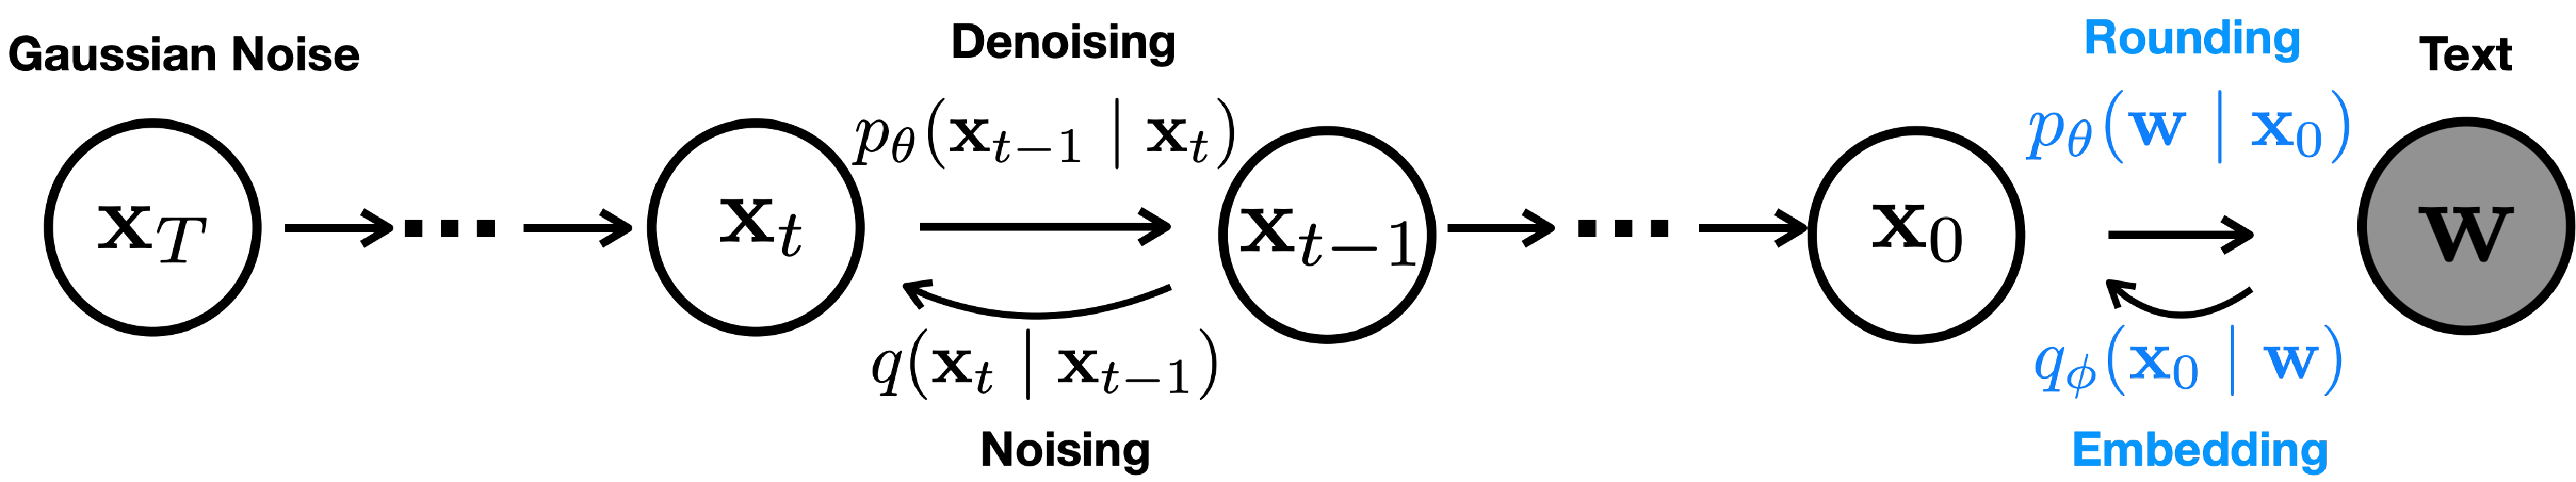
\includegraphics[width=0.8\textwidth]{fig/graphical_model_v2.pdf}
    \caption{\label{fig:graphical_model} A graphical model representing the forward and reverse diffusion processes. In addition to the original diffusion models \cite{ho2020denoising}, we add a Markov transition between $\cx{0}$ and $\ww$, and propose the embedding \cref{ssec:embeddings} and rounding \cref{ssec:rounding} techniques. }
\end{figure}

The diffusion model is trained to maximize the marginal likelihood of the data $\mathbb{E}_{\cx{0} \sim p_\text{data} }\log p_\theta(\cx{0})$, and the canonical objective is the variational lower bound of $\log p_\theta(\cx{0})$ \cite{pmlr-v37-sohl-dickstein15}:
\begin{equation}
\Lvlb (\cx{0}) = \mathop{\mathbb{E}}_{q(\cx{1:T} | \cx{0})} \left[\log \frac{q(\cx{T} | \cx{0})}{\ptheta(\cx{T})} + \sum_{t=2}^T \log \frac{q(\cx{t-1} | \cx{0},\cx{t})} {\ptheta(\cx{t-1} | \cx{t}) } - \log \ptheta( \cx{0} | \cx{1})\right].
\label{eqn:diffusion}
\end{equation}
However, this objective can be unstable and require many optimization tricks to stabilize \cite{nichol2021improved}. To circumvent this issue, \citet{ho2020denoising} devised a simple surrogate objective that reweights each terms in $\Lvlb$. In the $t$-th term of $\Lvlb$ we have 
\begin{equation}
\mathop{\mathbb{E}}_{q(\cx{1:T} | \cx{0})} \left[ \log \frac{q(\cx{t-1} | \cx{0},\cx{t})} {\ptheta(\cx{t-1} | \cx{t}) }\right] \propto \mathop{\mathbb{E}}_{q(\cx{1:T} | \cx{0})}  \left[ || \mu_\theta(\cx{t}, t) - \hat{\mu}(\cx{t}, \cx{0}) ||^2\right] + C, 
\label{eqn:simple}
\end{equation}
\pl{proportional to something plus a constant looks weird... is it really proportional to? the LHS isn't a probability so why can't we write = and a constant?}
where $C$ is a constant, $\hat{\mu}$ is the mean of the posterior
\pl{why does this depend on $\cx{0}$?} $q(\cx{t-1} | \cx{0},\cx{t})$, and $\mu_\theta$ is the mean of $\ptheta(\cx{t-1} \mid \cx{t})$ predicted by the diffusion model. Intuitively, this simplification matches the predicted mean of $\cx{t}$ to its true posterior mean. Applying this simplification for all terms in $\Lvlb$, we obtain $\Lsimple (\cx{0}) = \sum_{t=1}^T \mathbb{E}_{\cx{0}, \cx{t}} || \mu_\theta(\cx{t}, t) - \hat{\mu}(\cx{t}, \cx{0}) ||^2$.
\pl{you want displaymath this since this is the thing you use;
also there shouldn't be an extra $x_0$ in the subscript of the expectation, right since it's given?
}
While $\Lsimple$ is no longer a valid lower bound, but prior work found that it empirically made training more stable and improved sample quality \footnote{Our definition of $\Lsimple$ uses a different parametrization from \citet{ho2020denoising}. We define our squared loss in terms of $\mu_\theta(\cx{t}, t)$ while they express it in terms of $\epsilon_\theta(\cx{t}, t)$.}.
We will make use of similar simplifications in Diffusion-LM to stabilize training and improve sample quality (\cref{ssec:embeddings}).

\pl{if this is all review, can we trim this down and directly mention Lsimple? it seems like the details aren't really necessary here, and we should focus on what makes text unique, and say explicitly what we are taking over from vision wholesale and the properties; especially since Lsimple is intuitive, we can just declare that as the thing without deriving anything bout lower bounds since we don't have that anyway}

\pl{should also say what an example form is for $p_\theta$ just for concreteness}













\section{Diffusion-LM: Continuous Diffusion Language Modeling}
\label{sec:method}

Constructing Diffusion-LM requires several modification to the standard diffusion model.
First, we must define an embedding function that maps discrete text into a continuous space. To address this, we propose an end-to-end training objective for learning embeddings (\cref{ssec:embeddings}). 
Second, we require a rounding method to map vectors in embedding space back to words. To address this, we propose training and decoding time methods to facilitate rounding (\cref{ssec:rounding}). 
The two improvements make it possible to reliably train Diffusion-LMs, and we describe how to perform plug-and-play controllable generation on these models using classifier guidance (\cref{ssec:control_text}). 







\subsection{End-to-end Training} 
\label{ssec:embeddings}



To apply a continuous diffusion model to discrete text, we must \pl{-must} define an embedding function $\Emb(w_i)$ that maps each word to a vector in $\mathbb{R}^{d}$. We define the embedding of a sequence $\ww$ of length $n$ to be: $\Emb(\ww) = [\Emb(w_1), \dots, \Emb(w_n)] \in \mathbb{R}^{nd}$. 

We propose a modification of the diffusion model training objective (Equation \ref{eqn:diffusion}) that jointly learns the diffusion model's parameters and word embeddings.
In preliminary experiments, we explored random Gaussian embeddings, as well as pre-trained word embeddings \cite{pennington-etal-2014-glove, radford2019language}. We found that these fixed embeddings are suboptimal for Diffusion-LM compared to end-to-end training\footnote{While trainable embeddings perform best on control and generation tasks, we found that fixed embeddings onto the vocabulary simplex were helpful when optimizing for held-out perplexity. We leave discussion of this approach and perplexity results to \cref{app:simplex} as the focus of this work is generation quality and not perplexity.}.


As shown in Figure \ref{fig:graphical_model}, our approach adds a Markov transition from discrete words $\ww$ to $\cx{0}$ in the forward process, parametrized by $\qphi(\cx{0} | \ww) = \mathcal{N} (\Emb(\ww), \sigma_0 I )$. In the reverse process, we add a trainable rounding step, parametrized by $\ptheta(\ww \mid \cx{0}) = \prod_{i=1}^n \ptheta(w_i \mid x_i)$, where $\ptheta(w_i \mid x_i)$ is a softmax distribution. The training objectives introduced in \cref{sec:background} now becomes
\begin{equation}
\begin{aligned}
\mathcal{L}^\text{e2e}_{\text{vlb}} (\ww) &= \mathop{\mathbb{E}}_{q_\phi(\cx{0} | \ww)}\left[\mathcal{L}_{\text{vlb}} (\cx{0}) + \log \qphi(\cx{0} | \ww) - \log \ptheta(\ww | \cx{0})]\right], \\
 \mathcal{L}^\text{e2e}_\text{simple} (\ww) &= \mathop{\mathbb{E}}_{\qphi(\cx{0:T} | \ww)} \left[\Lsimple(\cx{0}) + || \cx{T}||^2 + || \Emb(\ww) - \xx_\theta(\cx{1}, 1) ||^2  - \log \ptheta(\ww | \cx{0})\right].
\end{aligned}
\label{obj:e2e}
\end{equation}
\pl{what's $x_\theta$? is this a typo?}

\begin{wrapfigure}[10]{R}{0.4\textwidth}
\vspace{-6mm}
\centering
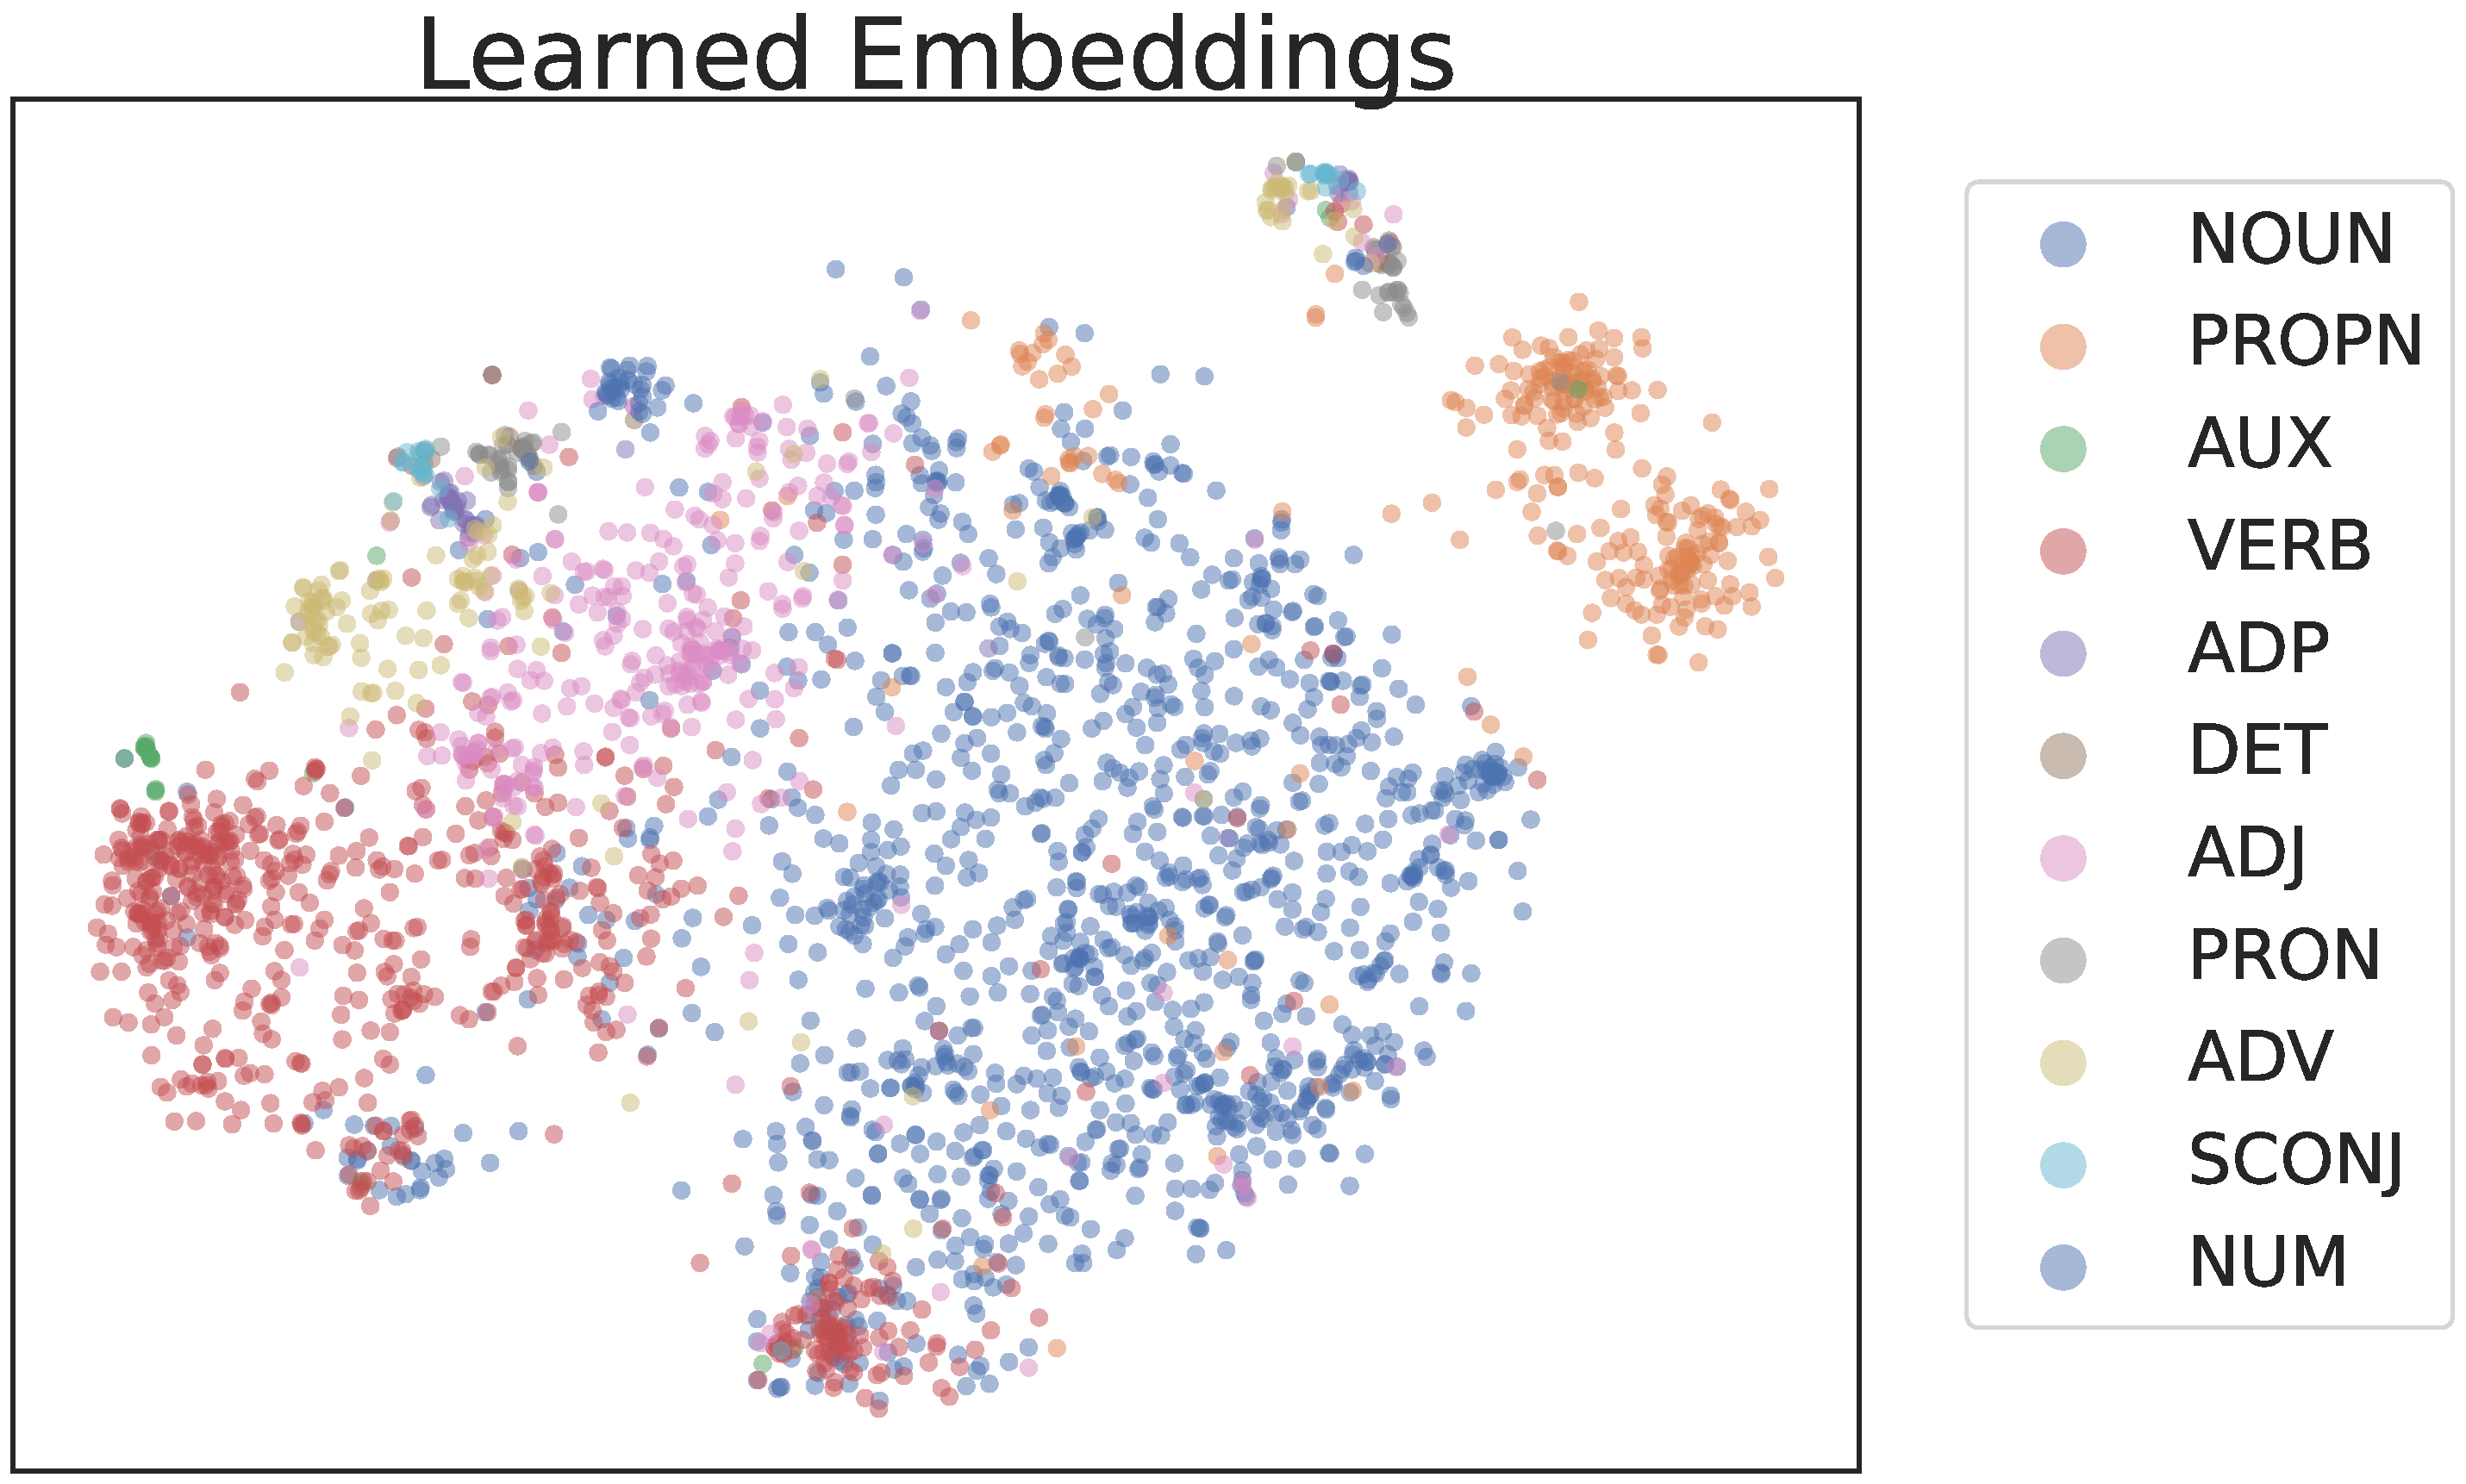
\includegraphics[width=\linewidth]{fig/embedding_128_v3.pdf}\caption{ \label{fig:emb} A t-SNE \cite{vanDerMaaten2008} plot of the learned word embeddings.}
\end{wrapfigure}

We derive $ \mathcal{L}^\text{e2e}_\text{simple} (\ww)$ from $\mathcal{L}^\text{e2e}_{\text{vlb}}(\ww)$ following the simplification in \cref{eqn:simple} and our derivation details are shown in \cref{app:derive}. Since we are training the embedding function, $q_\phi$ now contains trainable parameters and we use the reparametrization trick \citep{rezende2014stochastic, kingma2014auto} to backpropagate through this sampling step. 
Empirically, we find the learned embeddings cluster meaningfully: words with the same part-of-speech tags (syntactic role) tend to be clustered, as shown in \cref{fig:emb}. 



\subsection{Reducing Rounding Errors}
\label{ssec:rounding}

Even when we learn the embedding map, the rounding step \pl{what exactly is this?  This is really the key point of the paper - the thing that distinguishes text from vision, so take some time to explain it more} that maps a predicted word vector to its nearest word is prone to rounding errors.
Ideally, the denoising process itself should learn that the distribution over $\cx{0}$ is nearly a set of Dirac delta distributions, which would make the rounding step unambiguous. However, diffusion models do not seem to learn to perform rounding in practice, and there can be substantial ambiguity and rounding errors. Avoiding this requires that we predict more precise vectors before feeding it to the rounding step. 

One approach towards this goal is to parameterize the model to directly predict $\cx{0}$ at each diffusion step, as opposed to predicting the mean of $\cx{t-1}$ as derived in \cref{ssec:diffusion_setup}.  
Consequently, we modify $\Lsimple$ from $\sum_{t=1}^T || \mu_\theta(\cx{t}, t) - \hat{\mu}(\cx{t}, \cx{0}) ||^2$ to $\sum_{t=1}^T ||\xx_\theta(\cx{t}, t) - \cx{0} ||^2$, where we explicitly match $\xx_\theta(\cx{t}, t)$ and ground truth $\cx{0}$ \pl{don't know what this means}. 
These two parametrizations are both valid derivation from $\Lvlb$ (for derivation see \cref{app:derive}), but matching $\cx{0}$ is easier for the neural network to learn, therefore significantly reduces rounding error. 

Complementary to the training time parametrization, we also propose a decoding time technique that we call the \emph{clamping} trick. 
In the standard decoding approach, the model denoises $\cx{t}$ to $\cx{t-1}$ by first computing an
estimate of $\cx{0}$ via $\xx_\theta(\cx{t}, t)$, and sampling $\cx{t-1}$ conditioned on this estimate: $\cx{t-1} = \sqrt{\alphabar} \xx_\theta(\cx{t}, t) +\sqrt{1-\alphabar} \epsilon$, where $\alphabar_t = \prod_{s=0}^t (1-\beta_s)$ and $\epsilon \sim \mathcal{N}(0,I)$ \footnote{This follows from the marginal distribution $q(\cx{t} \mid \cx{0})$, which is a closed form Gaussian since all the Markov transitions are Gaussian.}. In the clamping trick, the model additionally maps the predicted vector $\xx_\theta(\cx{t}, t)$ to its nearest word embedding sequence. Now, the sampling step becomes $\cx{t-1} = \sqrt{\alphabar}\cdot \Clamp(\xx_\theta(\cx{t}, t)) +\sqrt{1-\alphabar} \epsilon$. The clamping trick forces the predicted embedding to commit to a word for intermediate diffusion steps, making the vector predictions more precise and reducing rounding errors.  

\pl{to be honest, I had trouble following this section;
given that this seems like the major technical contribution of the paper, I think it's worth expanding on things a bit and cutting down the general stuff about diffusions (which they can read another paper for)}
\pl{one thing that could help is at least stating what problem you're trying to fix (beyond the 'rounding is hard' problem) and intuitively why the approach is helpful}













